% This is "sig-alternate.tex" V2.1 April 2013
% This file should be compiled with V2.5 of "sig-alternate.cls" May 2012
%
% This example file demonstrates the use of the 'sig-alternate.cls'
% V2.5 LaTeX2e document class file. It is for those submitting
% articles to ACM Conference Proceedings WHO DO NOT WISH TO
% STRICTLY ADHERE TO THE SIGS (PUBS-BOARD-ENDORSED) STYLE.
% The 'sig-alternate.cls' file will produce a similar-looking,
% albeit, 'tighter' paper resulting in, invariably, fewer pages.
%
% ----------------------------------------------------------------------------------------------------------------
% This .tex file (and associated .cls V2.5) produces:
%       1) The Permission Statement
%       2) The Conference (location) Info information
%       3) The Copyright Line with ACM data
%       4) NO page numbers
%
% as against the acm_proc_article-sp.cls file which
% DOES NOT produce 1) thru' 3) above.
%
% Using 'sig-alternate.cls' you have control, however, from within
% the source .tex file, over both the CopyrightYear
% (defaulted to 200X) and the ACM Copyright Data
% (defaulted to X-XXXXX-XX-X/XX/XX).
% e.g.
% \CopyrightYear{2007} will cause 2007 to appear in the copyright line.
% \crdata{0-12345-67-8/90/12} will cause 0-12345-67-8/90/12 to appear in the copyright line.
%
% ---------------------------------------------------------------------------------------------------------------
% This .tex source is an example which *does* use
% the .bib file (from which the .bbl file % is produced).
% REMEMBER HOWEVER: After having produced the .bbl file,
% and prior to final submission, you *NEED* to 'insert'
% your .bbl file into your source .tex file so as to provide
% ONE 'self-contained' source file.
%
% ================= IF YOU HAVE QUESTIONS =======================
% Questions regarding the SIGS styles, SIGS policies and
% procedures, Conferences etc. should be sent to
% Adrienne Griscti (griscti@acm.org)
%
% Technical questions _only_ to
% Gerald Murray (murray@hq.acm.org)
% ===============================================================
%
% For tracking purposes - this is V2.0 - May 2012

\documentclass{sig-alternate-05-2015}
\usepackage{algpseudocode}
\usepackage{graphicx}
\usepackage{float}
\usepackage{subfigure}

\begin{document}

% Copyright
\setcopyright{none}
%\setcopyright{acmcopyright}
%\setcopyright{acmlicensed}
%\setcopyright{rightsretained}
%\setcopyright{usgov}
%\setcopyright{usgovmixed}
%\setcopyright{cagov}
%\setcopyright{cagovmixed}


% DOI
%\doi{10.475/123_4}

% ISBN
%\isbn{123-4567-24-567/08/06}

%Conference
%\conferenceinfo{PLDI '13}{June 16--19, 2013, Seattle, WA, USA}

%\acmPrice{\$15.00}

%
% --- Author Metadata here ---
%\conferenceinfo{WOODSTOCK}{'97 El Paso, Texas USA}
%\CopyrightYear{2007} % Allows default copyright year (20XX) to be over-ridden - IF NEED BE.
%\crdata{0-12345-67-8/90/01}  % Allows default copyright data (0-89791-88-6/97/05) to be over-ridden - IF NEED BE.
% --- End of Author Metadata ---

\title{Distributed LDA on Harp}
%
% You need the command \numberofauthors to handle the 'placement
% and alignment' of the authors beneath the title.
%
% For aesthetic reasons, we recommend 'three authors at a time'
% i.e. three 'name/affiliation blocks' be placed beneath the title.
%
% NOTE: You are NOT restricted in how many 'rows' of
% "name/affiliations" may appear. We just ask that you restrict
% the number of 'columns' to three.
%
% Because of the available 'opening page real-estate'
% we ask you to refrain from putting more than six authors
% (two rows with three columns) beneath the article title.
% More than six makes the first-page appear very cluttered indeed.
%
% Use the \alignauthor commands to handle the names
% and affiliations for an 'aesthetic maximum' of six authors.
% Add names, affiliations, addresses for
% the seventh etc. author(s) as the argument for the
% \additionalauthors command.
% These 'additional authors' will be output/set for you
% without further effort on your part as the last section in
% the body of your article BEFORE References or any Appendices.

\numberofauthors{8} %  in this sample file, there are a *total*
% of EIGHT authors. SIX appear on the 'first-page' (for formatting
% reasons) and the remaining two appear in the \additionalauthors section.
%
\author{
% You can go ahead and credit any number of authors here,
% e.g. one 'row of three' or two rows (consisting of one row of three
% and a second row of one, two or three).
%
% The command \alignauthor (no curly braces needed) should
% precede each author name, affiliation/snail-mail address and
% e-mail address. Additionally, tag each line of
% affiliation/address with \affaddr, and tag the
% e-mail address with \email.
%
% 1st. author
\alignauthor
Ethan Li\\
       \affaddr{School of Informatics and Computing}\\
       \affaddr{107 S. Indiana Avenue}\\
       \affaddr{Bloomington, Indiana}\\
       \email{li526@indiana.edu}
% 2nd. author
\alignauthor
Rohit Patil\\
       \affaddr{School of Informatics and Computing}\\
       \affaddr{107 S. Indiana Avenue}\\
       \affaddr{Bloomington, Indiana}\\
       \email{rnpatil@umail.iu.edu}
       }

% There's nothing stopping you putting the seventh, eighth, etc.
% author on the opening page (as the 'third row') but we ask,
% for aesthetic reasons that you place these 'additional authors'
% in the \additional authors block, viz.

% Just remember to make sure that the TOTAL number of authors
% is the number that will appear on the first page PLUS the
% number that will appear in the \additionalauthors section.

\maketitle
\begin{abstract}
\par
Harp LDA is a distributed variational bayes inference (VB) algorithm for LDA model which would be able to model a large and continuously expanding dataset using Harp collective communication library. We also study how variational bayes inference converges within Map-Collective jobs provided by Harp. The proposed algorithm is run against a corpus of Wikipedia Dataset to find if it can achieve better performance and shorter time and memory requirements. We also provide experimental procedures to evaluate execution accomplishment of our proposed algorithm in terms of scalability and log-likelihood metrics.
\end{abstract}


%
% The code below should be generated by the tool at
% http://dl.acm.org/ccs.cfm
% Please copy and paste the code instead of the example below. 
%
%\begin{CCSXML}
%<ccs2012>
 %<concept>
 % <concept_id>10010520.10010553.10010562</concept_id>
 % <concept_desc>Computer systems organization~Embedded systems</concept_desc>
 % <concept_significance>500</concept_significance>
% </concept>
% <concept>
%  <concept_id>10010520.10010575.10010755</concept_id>
%  <concept_desc>Computer systems organization~Redundancy</concept_desc>
%  <concept_significance>300</concept_significance>
% </concept>
% <concept>
%  <concept_id>10010520.10010553.10010554</concept_id>
%  <concept_desc>Computer systems organization~Robotics</concept_desc>
%  <concept_significance>100</concept_significance>
% </concept>
% <concept>
%  <concept_id>10003033.10003083.10003095</concept_id>
%  <concept_desc>Networks~Network reliability</concept_desc>
%  <concept_significance>100</concept_significance>
% </concept>
%</ccs2012>  
%\end{CCSXML}

\ccsdesc[500]{Computer systems organization~Distributed systems}
%\ccsdesc[300]{Computer systems organization~Redundancy}
%\ccsdesc{Computer systems organization~Robotics}
%\ccsdesc[100]{Networks~Network reliability}


%
% End generated code
%

%
%  Use this command to print the description
%
\printccsdesc

% We no longer use \terms command
%\terms{Theory}

\keywords{LDA; Harp; Distributed algorithm; Scalability}

\section{Introduction}     
Latent Dirichlet Allocation (LDA)\cite{blei2003latent}, a topic modeling algorithm designed for text documents in unsupervised environments. It is especially useful for web content such as on-line news articles, blogs along with data from major domains like Google, Yahoo, and Amazon etc. Suppose you have a very large corpus and want to come up with some inference about the data, topic models is a mechanism to get a corpus-level view of major themes. LDA assumes that the documents in a corpus are generated from a set of K topics. Thus from an input corpus and number of topics K, LDA model maps words in documents to topics. Even though the sequential model is theoretically effective, a significant drawback evident while using LDA is the amount of time taken and memory requirements for inference while dealing with a very large scaled and dynamically expanding corpus. Moreover the huge data-sets wont fit on a single machine. Thus a distributed multiprocessor system framework is essential for solving topic modelling LDA inference for a large data corpus. If suppose we have a distributed framework with will N processor, for distributed computation each of N processors deals with only 1/N of the total data set and the inference results of each processors are aggregated to generate the final results.
\par
Approximate inference for topic modelling using LDA can be carried out using a number of different approaches such as variational bayes methods, expectation maximization and Markov chain Monte Carlo methods. An approach discussed in Mr. LDA\cite{zhai2012mr} devised a parallel LDA algorithm in the Apache Hadoop framework\cite{white2012hadoop} using MapReduce programming framework. Mr. LDA approach also emphasized on positives of implementing variational inference over using Gibbs sampling (Markov chain Monte Carlo) in terms of extensibility, flexibility, and number of iterations and thus eventually affecting the scalability. Our proposed LDA model which is based on Harp\cite{zhang2015harp} collective communication library is similar to MapReduce framework and uses Variational Bayes (VB) inference. Although, MapReduce framework can provide better communication between multiple processors and high reliability systems, to might suffer from I/O cost to large number of HDFS read/write operations. Harp library can be plugged into Hadoop runtime to enable efficient in-memory communication to avoid HDFS read/write thus saving excess I/O cost. Moreover, other major plausible improvements of Harp comprises hierarchal data abstraction, collective communication model, pool based memory management, BSP style computation parallelism etc. A better understanding of our algorithm can be developed in the sections proposed methods and experimental results.

\section{Problem Definition}
LDA is a powerful topic modelling algorithm for clustering words into topics and documents into mixtures of topics. Even though the sequential LDA model is theoretically effective, a significant drawback evident while using LDA is the amount of time taken and memory requirements for inference while dealing with a very large scaled and dynamically expanding corpus. Moreover the huge data-sets won't fit on a single machine. Thus a distributed multiprocessor system framework is essential for solving topic modelling LDA inference for a large data corpus as an efficient way of distributing the computation across multiple machines. The primary aim of the project is to build a scalable topic modelling tool for a large corpus of textual data devised by implementing LDA model in a distributed environment. We follow the Mr. LDA to implement distributed variational bayes inference LDA on Harp. Harp modules particularly of our interests are dynamic scheduler, all-reduce and push-pull communication models.
\section{Proposed Method}

\begin{figure}[!htbp]
 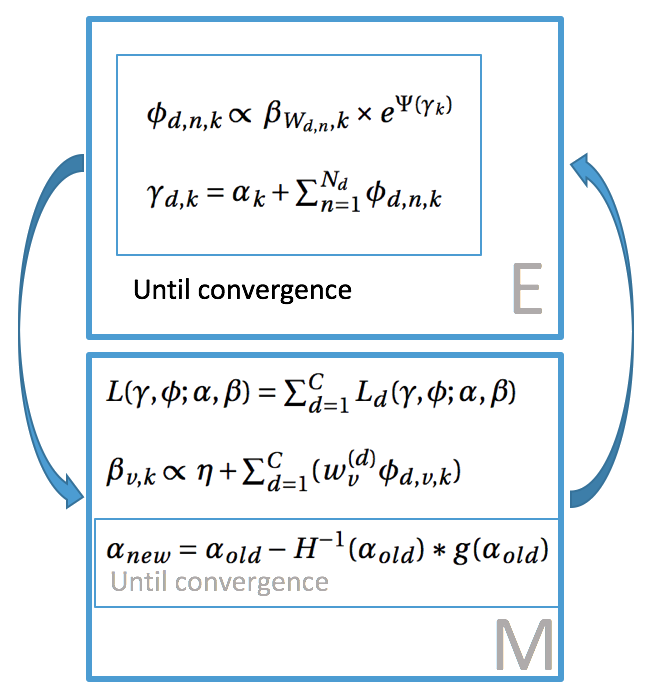
\includegraphics[width=0.45\textwidth]{reportCharts/algorithm_transparent}
  \caption{algorithm}
  \label{fig:algorithm_transparent}
\end{figure}

We propose a distributed LDA algorithm using Harp. First of all, the data will be preprocessed to be a D $\times$ V matrix M, where D is the number of documents in the corpus and V is the size of vocabulary. The element $M_{d,v}$  in the matrix is the number of tokens of the word v in the document d. Then the data will be partitioned to P partitions. Each partition contains D/P documents. P is the number of mappers. For each mapper, it will compute $\phi$, $\gamma$, $\alpha$, $\beta$ using VB method. The collective communication methods like \textit{allreduce} and \textit{push-pull} will be used to synchronize $\alpha$, $\beta$ and likelihood. The main pseudocode is as follows.

{\small
\begin{center}
\begin{algorithmic}[1]\label{HARP-LDA-MapCollective}
\State{\bf Pseudocode} \texttt{LDAMapCollective}
\State {\bf INPUT} ($inputDir$,  $metafile$, $outputDir$, \textsf<number of terms> $numOfTerms$, $numOfTopics$, $numOfDocs$,  $numOfMapTasks$, $numOfIterations$)
\State
\State \texttt{***}  $inputDir$ is the path to the data. In the $inputDir$, the data is splited into serval splits.
\State \texttt{***}  $metafile$ is the path to the metadata file. This file records the beginning doc index of each data splits.
\State \texttt{***}   $outputDir$ is the path to put the final results.
\State \texttt{***}   $numOfTerms$ is the size of the vocabulary.
\State \texttt{***}   $numOfTopics$ is the number of topics.
\State \texttt{***}   $numOfDocs$ is the number of documents in the dataset.
\State \texttt{***}   $numOfMapTasks$ is the number of mappers users want to launch.
\State \texttt{***}   $numOfIterations$ is the number of maximum running iterations.
\State parse Arguments
\State config a job
\State job.waitForCompletion()
\State {\bf return} 
\end{algorithmic}
\end{center}}


{\small
\begin{center}
\begin{algorithmic}[1]\label{HARP-LDA-MAPPER}
\State{\bf Pseudocode} \texttt{LDAMapper}
\State {\bf INPUT} (KeyValReader $reader$)
\State
\State \texttt{***}  $reader$ contains the paths to data files (splits)
\State
\State \texttt{***}  Data strutures following are:
\State \texttt{***}  \textbf{(Table)} $dataTable$ is a \textbf{numOfDocsInThisMapper  $\times$  numOfTerms} matrix
\State \texttt{***}  \textbf{(Table)} $alphaTable$  is a \textbf{1 $\times$  numOfTopics}  vector, represented by $\alpha$
\State \texttt{***}  \textbf{(Table)} $betaTable$ is a \textbf{numOfTerms  $\times$  numOfTopics} matrix, represented by $\beta$
\State \texttt{***}  \textbf{(Table)} $gammaTable$ is a \textbf{numOfDocs  $\times$  numOfTopics} matrix, represented by $\gamma$
\State \texttt{***}  \textbf{(Table)} $phiTable$ is a \textbf{numOfTerms  $\times$  numOfTopics} matrix, represented by $\phi$
\State \texttt{***}  \textbf{(Table)} $globalPhiTable$ is a \textbf{numOfTerms  $\times$  numOfTopics} matrix
\State \texttt{***}  \textbf{(Table)} $localPhiTable$ is a \textbf{numOfTerms  $\times$  numOfTopics} matrix
\State \texttt{***}  \textbf{(Table)} $totalAlphaSufficientStatisticsTable$  is a \textbf{1 $\times$  numOfTopics}  vector
\State
\State load data from $reader$ to \textbf{(Table)} $dataTable$
\State initialize  \textbf{(Table)} $alphaTable$, $betaTable$
\Repeat
\For {doc d in dataTable}
\State compute loglikelihooodAlphaInOneDoc
\State initialize $\gamma$
\State \texttt{***}  E-step, train $\gamma$ and  $\phi$
\State \texttt{***}  also compute loglikelihoodPhiInOneDoc
\Repeat
\For{ v in vocabulary}
\For { k in topics}
\State $\phi_{v,k} = \beta_{v,k} \times  \exp(\Psi(\gamma_{d,k}))$
\EndFor
\State normalize row $\phi_{v,*}$
\State \texttt{***} $w_v$ is the value of dataTable(d, v), which is the count of the tokens of word v in doc d.
\State update $\sigma = \sigma + w_v\phi_v$
\EndFor
\State update $\gamma_{d,*} = \alpha + \sigma$
\Until convergence
\State compute loglikelihoodGammaInOneDoc
\State LogLikelihood += likelihoodAlphaInOneDoc + likelihoodGammaInOneDoc + likelihoodPhiInOneDoc;
\State update totalAlphaSufficientStatistics
\State aggregate $\phi$ to $localPhiTable$
\EndFor
\State
\State \texttt{***}  M-step, update alpha and beta
\State \texttt{***}  compute $\beta$
\State \textbf{push} data from localPhiTable to globalPhiTable
\State normalize data in globalPhiTable
\State \textbf{pull} data from globalPhiTable to localPhiTable
\State update new $\beta$ from localPhiTable
\State
\State \texttt{***}  compute $\alpha$
\State \textbf{allreduce} totalAlphaSufficientStatistics
\State compute $\alpha$ using Newton-Raphson method (need totalAlphaSufficientStatistics vector)
\State
\State
\State \texttt{***}  compute loglikelihood
\State \textbf{allreduce} loglikehood
\Until  loglikehood converges or reach the maximum iterations
\State output results
\State {\bf return} 
\end{algorithmic}
\end{center}}

The workflow can be found in figure~\ref{fig:workflow_transparent}. Multiple techniques are used to gain good scalability and speed.

\begin{itemize}
\item{\textbf{Data preprocessing and compression.}}Data preprocessing involved filtering common English stop words, stemming words to origin and removing non-alphanumeric words. We used Apache Lucene library\cite{cutting2008apache} to devise the data preprocessing. Since the data is sparse, we adopt sparse matrix format to compress the dataset. It only stores (word\_id:numOfOccurrence) pairs. For example, a dataset is as in table \ref{tab:data}. After removing the stop words and stemming words to origin, we can get word-id pairs in table \ref{tab:pairs}. The general option is to map this dataset to matrix, like in table \ref{tab:matrix}. There are many zeros in table \ref{tab:matrix}. To save memory space, our sparse matrix format for this dataset is in table \ref{tab:sparse}.

\begin{table}[!htbp]
\begin{center}
\begin{tabular}{c|c}\hline
doc\_id & text \\ \hline \hline
doc\_0 & I love programming.\\ \hline
doc\_2 & Smith is working. \\ \hline
doc\_2 & Harp is a collective library. \\ \hline
\end{tabular}
\end{center}
\caption{a sample dataset}
\label{tab:data}
\end{table}

\begin{table}[!htbp]
\begin{center}
\begin{tabular}{c|c|c|c}\hline
word & id & word & id \\ \hline  
I & 0  &  work & 4 \\ 
love & 1& harp & 5\\  
program & 2 &  collective & 6  \\  
smith & 3 & library & 7 \\ \hline
\end{tabular}
\end{center}
\caption{word-id pairs}
\label{tab:pairs}
\end{table}

\begin{table}[!htbp]
\begin{center}
\begin{tabular}{ccccccccc}\hline\hline
 1 & 1 & 1 & 0 & 0 & 0 & 0 & 0  \\ 
 0 & 0 & 0 & 1 & 1 & 0 & 0 & 0  \\ 
 0 & 0 & 0 & 0 & 0 & 1 & 1 & 1 \\ \hline\hline
\end{tabular}
\end{center}
\caption{matrix representation}
\label{tab:matrix}
\end{table}

\begin{table}[!htbp]
\begin{center}
\begin{tabular}{ccccccccc}\hline\hline
 0:1 & 1:1 & 2:1  \\ 
 3:1 & 4:1 \\ 
 5:1 & 6:1 & 7:1 \\ \hline\hline
\end{tabular}
\end{center}
\caption{sparse matrix representation}
\label{tab:sparse}
\end{table}

\item{\textbf{Load balancing.}}

Load balance is important in distributed environment because it will reduce the waiting time. For example, if the algorithm is running on two machines. Machine1 takes 10\% of the data and machine2 takes 90\% of the data, machine1 will have to keep waiting until machine2 finishes it's work. The best case is that all machines finishing their computation at the same time and no waiting happens. We use two nodes in our experiments. So we partition the data into two partitions. Each partition contains the same number of documents. Besides, in the partition procedure, we keep the number of (word\_id: numOfOccurrence) pairs similar in these two partitions. So each node will do similar amount of computation.

\item{\textbf{Dynamic scheduling.}}
We adopt harp's dynamic scheduling scheme to further divide the computation on thread level. For example, we launch 16 threads in each machine. Then every thread will take one document  every time and do similar computation. Then after all documents are processed, the results from these threads will be aggregated to get the full model data.

\item{\textbf{Collective communication.}}
The computations are divided into multiple nodes. So it's necessary to do synchronization after computations. In our case, we will need to synchronize $\phi$ and $\alpha$ sufficient statistics ($\alpha'$ in figure~\ref{fig:workflow_transparent}). $\alpha'$ is a 1-dimensional vector and will be needed in every node. So allreduce communication scheme provided by harp is applied. $\phi$ is instead a matrix of words vs topics. It's a numOfTerms by numOfTopics matrix. It's not scalable to use allreduce for synchronizing this matrix because every node will store the whole matrix, which will be a bottleneck if the dataset is large.  Also the communication overhead is very high. Notice that some words are not actually in some particular partitions. So the $\phi$ matrix in specific nodes is a numOfTermsInThisPartition by numOfTopics matrix. numOfTermsInThisPartition can be much smaller than numOfTerms. So push-pull communication scheme is more scalable for synchronizing this matrix.

\end{itemize}

\begin{figure}[!htbp]
 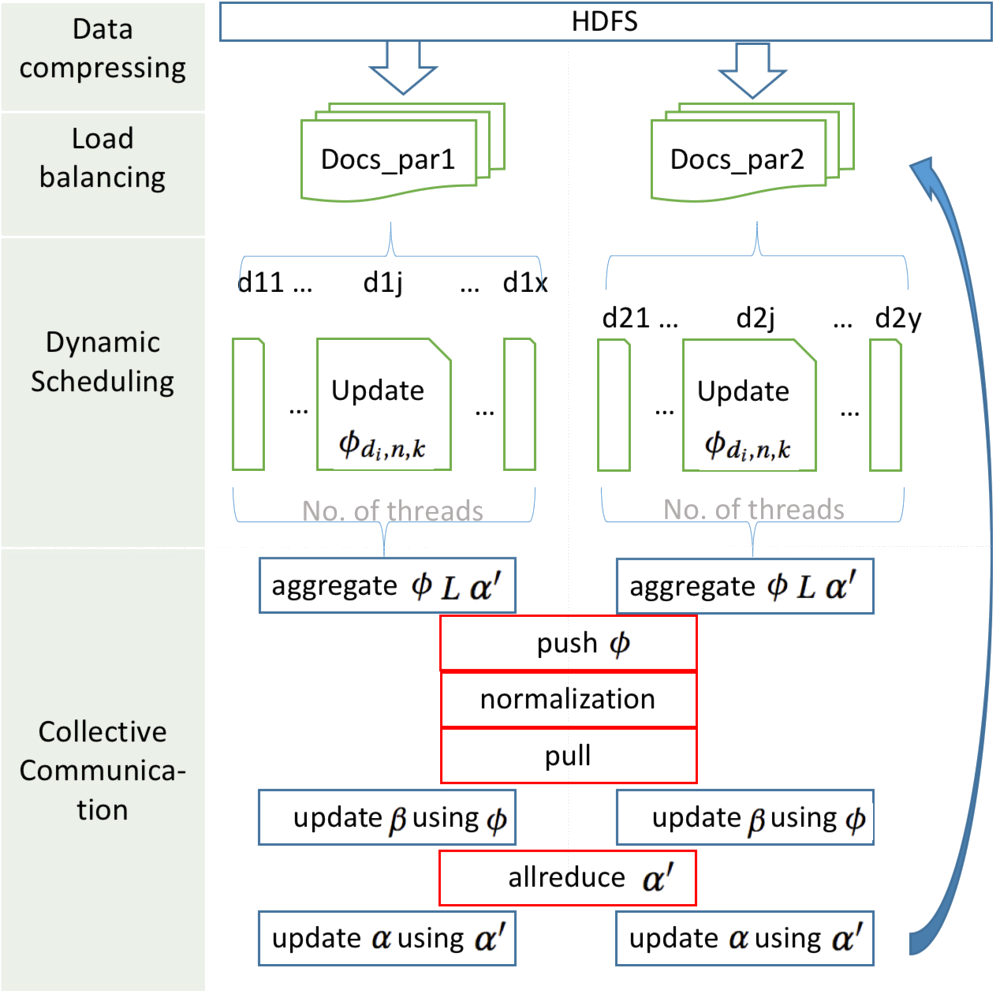
\includegraphics[width=0.45\textwidth]{reportCharts/workflow_transparent}
  \caption{workflow}
  \label{fig:workflow_transparent}
\end{figure}

\begin{figure*} [!htbp]
\centering
\subfigure[]{ \label{fig:convergence:a} 
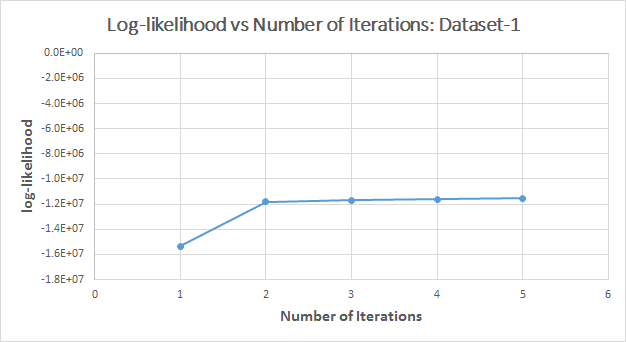
\includegraphics[width=2.0in]{reportCharts/data1-iterations.png}} 
\hspace{0.1in} 
\subfigure[]{ \label{fig:convergence:b}
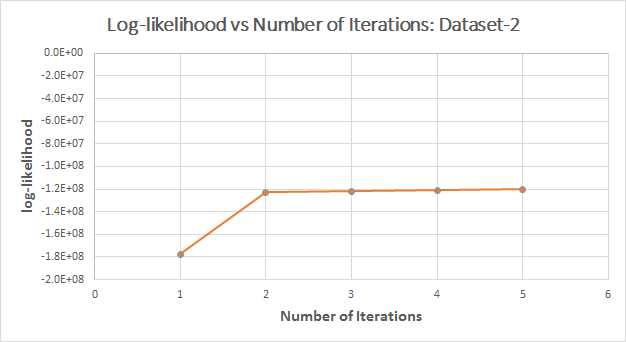
\includegraphics[width=2.0in]{reportCharts/data2-iterations.png}} 
\hspace{0.1in} 
\subfigure[]{ \label{fig:convergence:c}
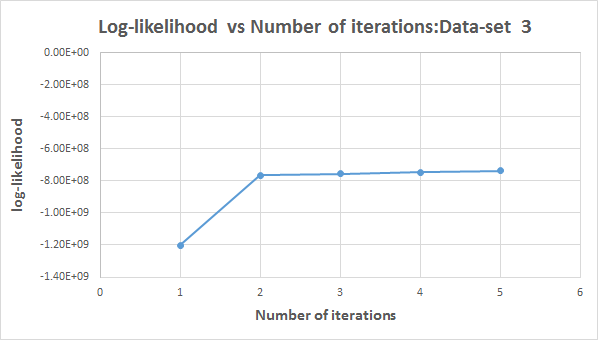
\includegraphics[width=2.0in]{reportCharts/data3-iterations.png}} 
\hspace{0.1in} 
\subfigure[]{ \label{fig:convergence:d}
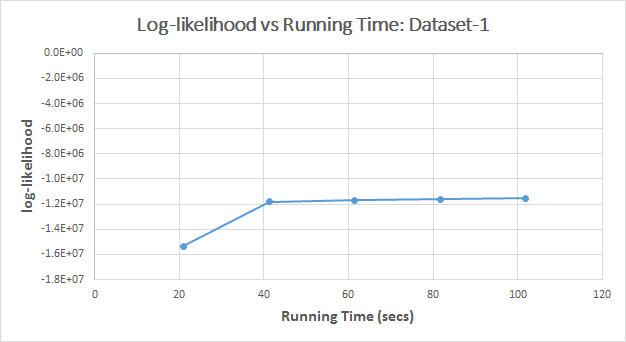
\includegraphics[width=2.0in]{reportCharts/data1-time.png}} 
\hspace{0.1in} 
\subfigure[]{ \label{fig:convergence:e}
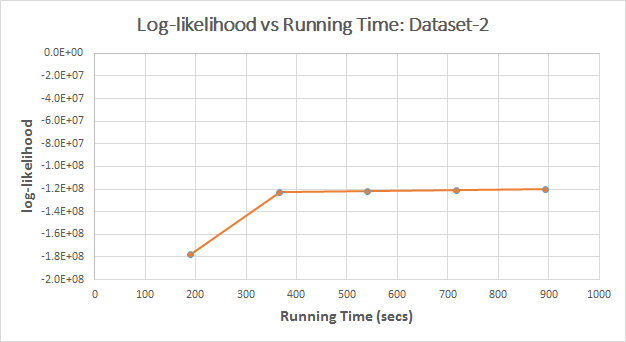
\includegraphics[width=2.0in]{reportCharts/data2-time.png}} 
\hspace{0.1in} 
\subfigure[]{ \label{fig:convergence:f}
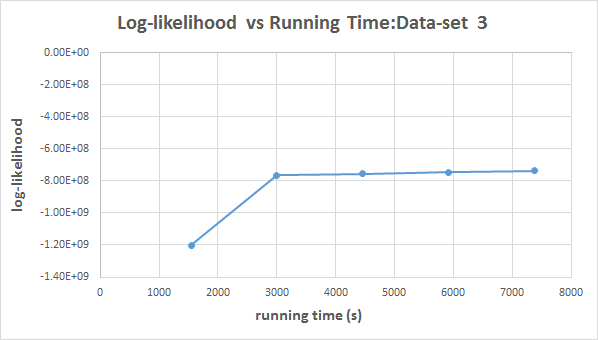
\includegraphics[width=2.0in]{reportCharts/data3-time.png}} 
\caption{Evaluation of convergence}
\label{fig:convergence} 
\end{figure*}
 
 

 
\section{Experiments}\label{experiments}
We worked on a Wikipedia dataset dump file. The total size of file was ~12 GB. For our experimental procedures we samples the corpus into 3 sub-samples from the Wikipedia dataset. The details of the datasets are shown in table~\ref{tab:datasets}. We ran our experiments on Juliet Cluster with 2 allocated nodes and a maximum thread count of 16 threads. The number of topics in these experiments is fixed to be 100.
\begin{table}[!htbp]
\begin{center}
\begin{tabular}{c|c|c|c}\hline
Name             & Dataset-1  & Dataset-2 & Dataset-3 \\ \hline\hline
docsize           & 744           & 7698   & 80986 \\ \hline
numOfWords  & 89907       & 435840  & 1454666 \\ \hline
numOfTokens & 535156     & 5308848 &  36096582 \\ \hline
\end{tabular}
\end{center}
\caption{datasets}
\label{tab:datasets}
\end{table}



\subsection{Evaluation of convergence}
An important metric for evaluation of our LDA model is log-likelihood. We conducted a series of experiments on increasing the size of the input data-sets (1k, 10k and 100k). For each experiment, 16 threads per node are launched.

The results in figure~\ref{fig:convergence} provide an evidence depicting the log-likelihood results of Harp-LDA against the incrementing number of iterations and the noted running time. A clear indication of fast convergence of likelihood after a few number of iterations is observed.  



\subsection{Evaluation of scalability}
The primary motivation for developing distributed algorithms for LDA is to have high scalable model in terms of memory and running time. Memory requirements depend on both memory for data and memory for model parameters. The variational LDA requires a few number of iterations to  converge. Fewer iterations means less frequency of communication. The experiments for the evaluation of scalability of the proposed LDA model ensured by two measures viz. increasing the size of data-set and increasing the number of parallel threads running. We conducted a series of experiments on increasing the size of the input data-sets (1k, 10k and 100k). For each data set we gradually increased the number of parallel threads over a range of (1, 2, 4, 8 and 16). The results are shown in figure~\ref{fig:speedup} and figure~\ref{fig:scalability}.

Two primary observations for these experiments were: 
\begin{itemize}
\item \textbf{Scalability by data volume.}
For each data-set increasing number of threads show a nearly linear growth in the speed up for the proposed LDA model. This depicts high scalability.
\item \textbf{Scale up.} By increasing the number of thread per node, the nearly linear decrease of running time is observed.
\end{itemize}

\begin{figure}[!htbp]
 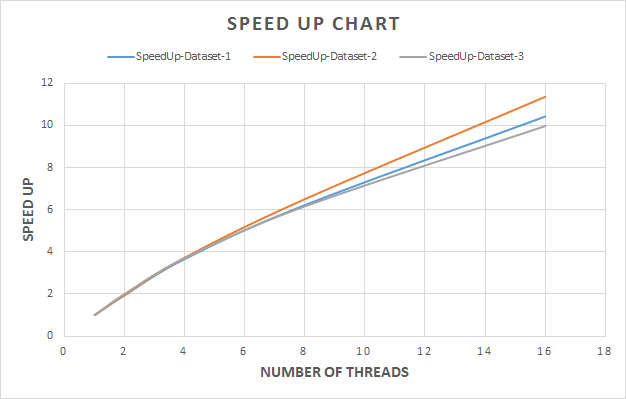
\includegraphics[width=0.45\textwidth]{reportCharts/speedup}
  \caption{speedup}
  \label{fig:speedup}
\end{figure}



\begin{figure*}[!htbp]
\centering
\subfigure[]{ \label{fig:scalability:a} 
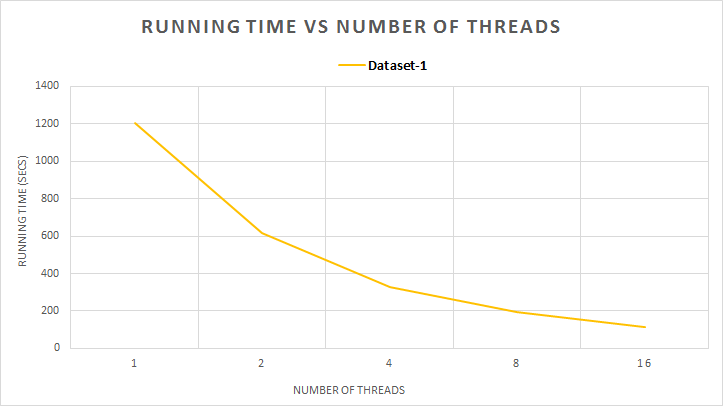
\includegraphics[width=2.0in]{reportCharts/numberofThreads-data1.png}} 
\hspace{0.1in} 
\subfigure[]{ \label{fig:scalability:b}
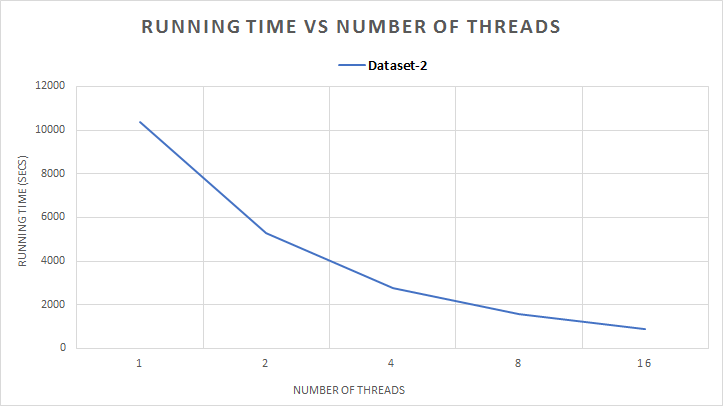
\includegraphics[width=2.0in]{reportCharts/numberofThreads-data2.png}} 
\hspace{0.1in} 
\subfigure[]{ \label{fig:scalability:c}
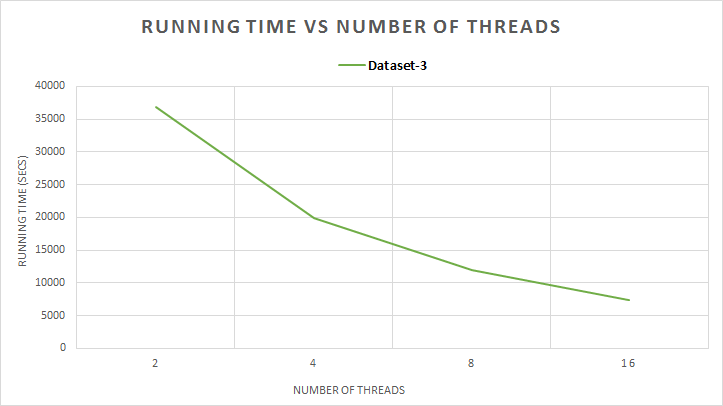
\includegraphics[width=2.0in]{reportCharts/numberofThreads-data3.png}} 
\caption{Evaluation of scalability}
\label{fig:scalability} 
\end{figure*}


\section{Conclusions} %\end{document}  % This is where a 'short' article might terminate
We proposed distributed LDA algorithm based on Harp. It represents a scalable mechanisms for inference of topic models. Our proposed LDA model based on Harp collective communication library enables efficient in-memory communication to avoid any excess HDFS read/write thus saving I/O cost. We also adopt specific data format, load balancing scheme, dynamic scheduling to achieve good performance and less memory requirements. The results  from the experimental procedure on Wikipedia Dataset suggests clear scope of fast convergence and high scalability. 

The limited time and resources of the project obstructs us from testing our algorithm more thoroughly. In the future, we will apply our algorithm to larger datasets and use more machines to verify the performance in real big data environment. And we will also find counterparts to do comparison in terms of scalability, convergence speed and accuracy measures.


%ACKNOWLEDGMENTS are optional
\section{Acknowledgments}
We thank Professor Judy Qiu, Bingjing Zhang, Po Peng and AI's help.

%
% The following two commands are all you need in the
% initial runs of your .tex file to
% produce the bibliography for the citations in your paper.
\bibliographystyle{abbrv}
\bibliography{distributedlda}  % sigproc.bib is the name of the Bibliography in this case
% You must have a proper ".bib" file
%  and remember to run:
% latex bibtex latex latex
% to resolve all references
%
% ACM needs 'a single self-contained file'!
%
%APPENDICES are optional
%\balancecolumns
%\appendix
%Appendix A \subsubsection{Theorem-like Constructs}
 

%\balancecolumns % GM June 2007
% That's all folks!
\end{document}
